\documentclass[12pt]{article}

\usepackage{fullpage}
\usepackage{floatrow}
\usepackage{fourier}
\usepackage{parskip}% http://ctan.org/pkg/parskip
\usepackage{graphicx}
\usepackage[labelfont={bf},margin=1cm]{caption}
\usepackage{subcaption}
\usepackage{textcomp}
\usepackage{amsmath} %larger fractions
%\usepackage[round,authoryear]{natbib}
\usepackage[utf8]{inputenc}
\usepackage[backend=biber,citestyle=authoryear,bibstyle=authoryear,maxbibnames=10]{biblatex}
\addbibresource{VCPbibliography.bib}

\AtEveryBibitem{ %
	\clearfield{url} %
	\clearfield{ISSN} %
	\clearfield{ISBN} %
}


%\usepackage{hyperref}

\begin{document}
%Ignore this page, it's so I can have a reference for the different citation formats and will be removed before turning in the paper.
%
%
%cite \cite{buckland2001} \cite{komodo2013} \\
%cite* \cite*{buckland2001} \cite*{komodo2013}\\
%parencite \parencite{buckland2001} \parencite{komodo2013}\\
%parencite* \parencite*{buckland2001} \parencite*{komodo2013}\\
%textcite \textcite{buckland2001} \textcite{komodo2013}\\
%smartcite - does the super script/foot note thing.
%\newpage
\begingroup  
  \centering
  \LARGE Masters Report - Variable Circular Plots: Station Placement and the Independence Assumption\\[1em]
  \large Matt Edwards\\
 % 26 May 2014\par
  \today\par
\endgroup

\section{Introduction}
Estimating population density of plants or animals is a persistent issue in the ecological sciences. Distance sampling, in the form of line and point transects (alternatively, Variable Circular Plots (VCP)), is a common estimation method. They are useful when individual objects are too small to be seen from the air or may be masked by the canopy (birds, small animals, ground plants, etc.).

Distance sampling has been around since the early 1900s. In the 1970s, more rigorous scientific methods were applied, including papers by Ramsey and Scott \parencite*{ramsey1979,ramsey1981} which augmented work done by Emlen in 1971. \cite{burnham1980} is a monograph on the theory and application of line transect sampling. Non-parametric methods have been examined by \textcite{quang1993,mack1998}, among others. Distance sampling continues to be used and modified, combined with mark-recapture methods \parencite{laake2011}, extended for use with underwater acoustics for estimates of krill populations \parencite{krill2011}, and a study by \textcite{camera2011} combines distance sampling with camera traps to estimate populations. For a more in-depth discussion of the history of distance sampling see \textcite{buckland2001}. 

Recent studies that use distance sampling include Norwegian bird populations \parencite{pedersen2012}, Komodo dragon prey estimates \parencite{komodo2013}, Serengeti carnivore abundance \parencite{serengeti2011}, and estimates for butterfly populations \parencite{butterfly2011}. 

With Line Transects, a (straight) line is randomly placed in the study area, then walked by the observer, with any objects of interest noted and the distance perpendicular to the transect recorded. With point transects, the observer stands in one spot, recording the direct line distance from herself to the object of interest as if it was projected on the ground, within the 360\textdegree. This results in data similar to the line transect, but with more safety for the observer as they do not have to watch for moving wildlife at the same time as navigating potentially treacherous terrain. \cite{ramsey1979}.

With line transects, animals may react to an observer moving through the area by hiding or moving away. If the observer is standing still, and has allowed a ``cooling'' period for things to return to normal--possible with point transects--animal behavior may be more natural and less influenced by the presence of the observer.

Observations of objects can take the form of visual sightings or detection of auditory cues, or one confirmed by the other, as long as an accurate distance can be measured.

\textcite{buckland2001} draws a distinction between point transects, where only the area immediately surrounding the point is surveyed (area of estimated perfect detectability), and Variable Circular Plots, where a census is taken of the area $\pi w^2$, where $w$ is the furthest distance at which there is a possibility of observing the object of interest. However, in \textcite{buckland2006, quang1993} the terms are used interchangeably. They will be used interchangeably here also, with the understanding this paper addresses the second type, where an area of $\pi w^2$ is censused.

Objects closer to the observer are typically easier to spot than objects further away. Considering the probability of detecting an object, we can imagine that there is an area of (nearly) perfect detectability near the observer, that drops off the further away from the observer the object is. This detectability function, defined as the probability of detecting an object, given that it is at distance $r$ is labeled $g(r)$, with $r$ being the observation distance. If no other covariates are tracked, we end up with a count of objects observed, and the distances from the line or point at which they were observed.

It is preferable for the detection function, $g(r)$, to have a "shoulder" at 0, where the probability of detection is 1. A half-normal curve, scaled such that $g(0)=1$ is an example \parencite{buckland2001}.

An estimate of population density is $n$, the count of objects observed, divided by the area in which they were observed, times the probability of observing the object at that distance. \cite{buckland2001} %eq 2.12, pg 39

$\hat{D}=n/(\mbox{Area})*P(\mbox{observing object}|\mbox{distance }r)$

The difficulty in distance sampling comes from estimating $g(r)$. Many methods have been proposed, all with their pros and cons. This paper concentrates on the kernel method, as detailed by \textcite{quang1993}. This is a non-parametric method, using the kernel of a normal distribution to obtain a kind of ``average observation distance'' to be used in the calculation of the effective area surveyed for our population density estimate.

\section{Micronesian Bird Data}
\begin{figure}
	\caption{Aggregated Collared Kingfisher Observation Distances, Rota \& Tinian, 20 m bins: \cite{micronesian}}
	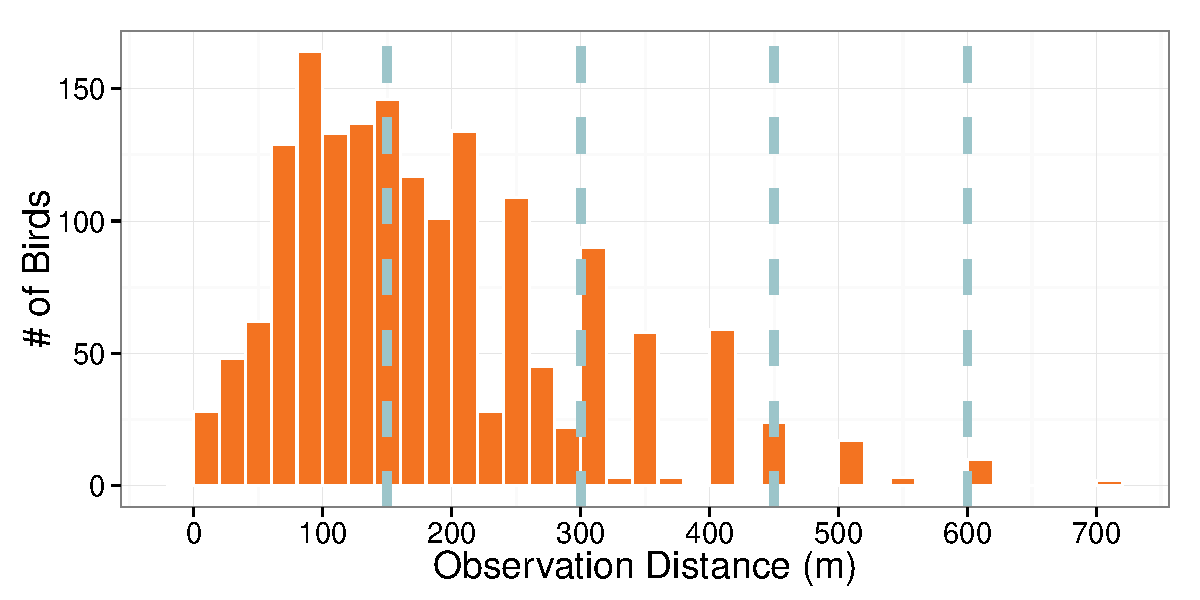
\includegraphics[width=\textwidth]{../images/histogram_dist_20m.pdf}
	\label{fig:82dist}
\end{figure}
The ``Micronesian Forest Bird Survey'' by \textcite{micronesian} is a work using Variable Circular Plots (VCPs) placed using a random-systematic transect design to monitor the density of several bird species in the Micronesian islands.

Each of the five islands included in the survey was divided into regions. Initial transects were given random positions and angles, with subsequent transects placed parallel, 2km apart (the ``random-systematic'' method). Stations were placed every 150m along the transects. Two observers, standing 20 m apart, would wait several minutes for the wildlife to quiet down after their arrival, and then spend 8 minutes noting any birds they could detect either visually or aurally. Distance and species were noted, as well as other covariates such as foliage density, and weather conditions. 

Figure~\ref{fig:82dist} illustrates the distance data for the Collared Kingfisher. This data represents the aggregated data from two islands, Tinian and Rota, and all four observers. We can observe several things in this plot:

First, there are very low counts of birds immediately around the station, a peak at around 100 m, a fairly level section from 100--200 m, and a drop off after 200 m. This would seem to indicate that the presence of the observers caused either movement away from the station (the crest around 100 m) or alternatively a suppression of vocalizations and/or movement directly around the station. 

Secondly, the further away from the station, the distance observations were heaped into convenient distances. With smaller bin widths, this is also evident in the 100--200 m range as well.

Lastly, note that the detection distances are high between 100--200 m, and recall that the stations were placed 150 m apart. Since the stations on a transect were generally visited in sequence, this means it is possible a bird could have been observed from more than one station. How does this affect the independence of our observations? Will it make a difference in our final population density estimates?

\subsection{Independence}
Both \textcite{ramsey1979,buckland1987} discuss the assumption that the VCPs are placed randomly through the study area. This would seem to implicitly state that their observational ranges might by chance overlap, meaning a single object of interest could be observed from more than one station.  \textcite[240]{thompson2012} likewise indicates random placement of line transects which would seem to allow for a potential overlap of observation zones. 

\textcite{buckland2001} discuss the random placement of both line and point transects, without addressing the potential for sightings to overlap. \textcite{reynolds1980} state that the possibility of observing the same bird from two stations should be avoided. \textcite{buckland2006} says simulations showed that analysis was robust to violations of independence (meaning overlap, or multiple observations on same object).

\textcite[233]{buckland2001} discuss that each line or point must be ``randomly and independently located,'' with ``an equal probability of selection'' for all portions of the study area.

\textcite[235]{buckland2001} states ``Transects are normally spaced at a sufficient distance to avoid detecting an object from two neighboring transacts, although this is not usually critical unless sampling a line changes the animal distribution at neighboring, as yet unsampled lines.''

They do state that for random-systematic transects, the methodology used by \textcite{micronesian}, that each transect line should be treated and analyzed as a cluster.

In discussing line transects, \textcite{barry2001} treats it as a two-stage sample, with non-unique clusters (each study object can be in more than one cluster) having an equal probability of selection. This would seem to (but does not explicitly) endorse the possibility of overlapping VCPs. 

One of the assumptions of distance sampling is that the objects being studied are distributed homogeneously with some uniform density, $D$, throughout the space \textcite{ramsey1981}.  (If the data is clustered we have other problems, not addressed here.) If the uniform distribution is the case, then it would make sense that it should not matter if the observations overlap, as long as the act of observing at one station does not affect the observations at the neighboring station. This echoes Buckland’s statement a few paragraphs previous.

\textcite[244]{thompson2012} mentions that the systematic selection of transects (random position of first, with additional transects a fixed distance apart) does not affect the approximate unbiasedness of the density estimator, but will have an effect on the approximate unbiasedness of the variance estimator. 

It is clear the literature is divided on whether or not our observation areas should overlap. VCP layouts similar to \textcite{micronesian} ``random-systematic'' layout are common in the literature.

\subsection{Bias \& Consistency}
\textcite{buckland2001,ramsey1979} Buckland et al. (2001) and Ramsey \& Scott (1970) both claim that if our detectability estimate $g(z)=$1 out to $r$, then $\hat{D}$ is unbiased. 

\textcite{barry2001} compared design-based and  model-based estimates of density and variance. (Their focus was line transects, but they state it is analogous to point transects and the conclusions should carry across.) They concluded that model-based estimates were unbiased if and only if the assumptions of objects being independent and uniformly located held. They noted that, in practice, this is probably not a feasible assumption. For design-based inference, they caution about both the density and variance estimates.

\textcite{roeder1987} use simulations to demonstrate that no method is completely applicable in 100\% of situations, and will go wrong at some point, depending on the specific conditions.

The overall conclusion is that, if all assumptions hold, density estimates using VCPs are unbiased and reasonably consistent. In practice, however, having the assumptions actually hold true is a precarious proposition. The appropriate estimation of $g(r)$ will vary depending on the specific situation, and it is up to the scientist and statistician to understand the data and choose the best approach.

\section{Simulation}
As was discussed in the previous section, the issue of independence of the point transects does not have a consensus in the literature. If independence is required for proper estimation, then the random-systematic placement (hereafter, ``transect'') layout may require some adjustment of the estimate to bring it in line with survey layouts where the observations areas do not overlap.

Through simulation, we can explore what happens under different VCP placement schemes, detection densities, and object movement amounts, and compare the resulting density estimates to their known values to evaluate the performance of the estimators.

\subsection{VCP Arrangement}
\label{sec:layout}
To examine the effect of VCP overlap, we will look at three options for VCP arrangement:
\begin{itemize}
	\item Structured: VCPs placed so that observation distances do not overlap
	\item Random: VCPs placed completely at random
	\item Transect: Two transects of 18 stations each, placed according to \textcite{micronesian} design: 150 m between stations, 2 km distance between parallel transects.
\end{itemize}
\begin{figure}
	\centering

	\begin{subfigure}[b]{0.45\textwidth}
		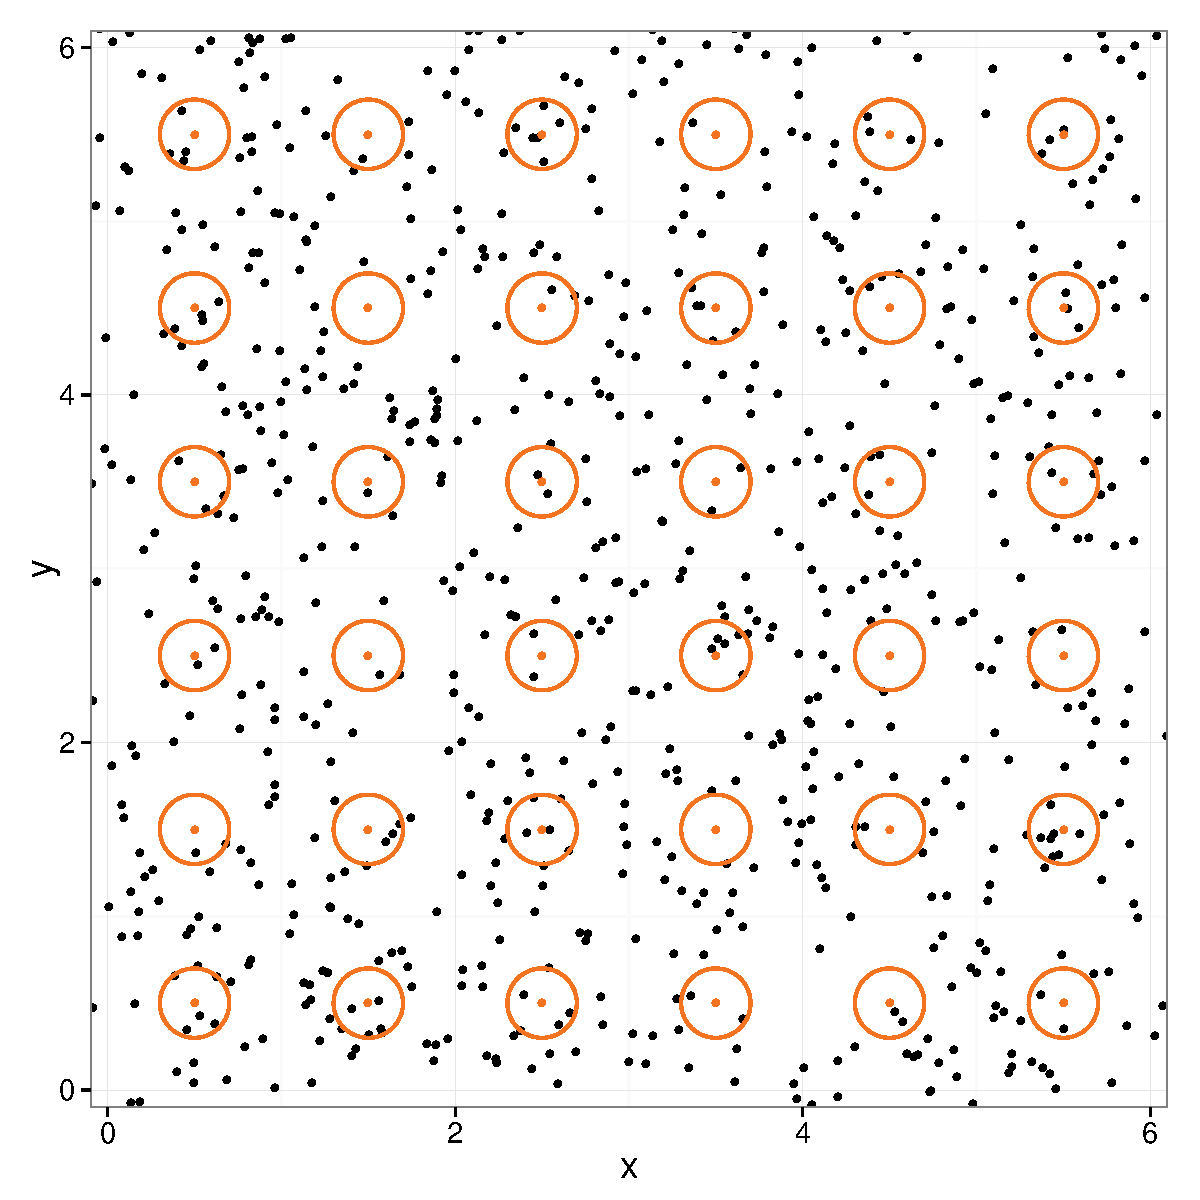
\includegraphics[width=\textwidth]{../images/layout_structured.pdf}
		\caption{Structured Layout}
		\label{fig:structured}
	\end{subfigure}
	\begin{subfigure}[b]{0.45\textwidth}
		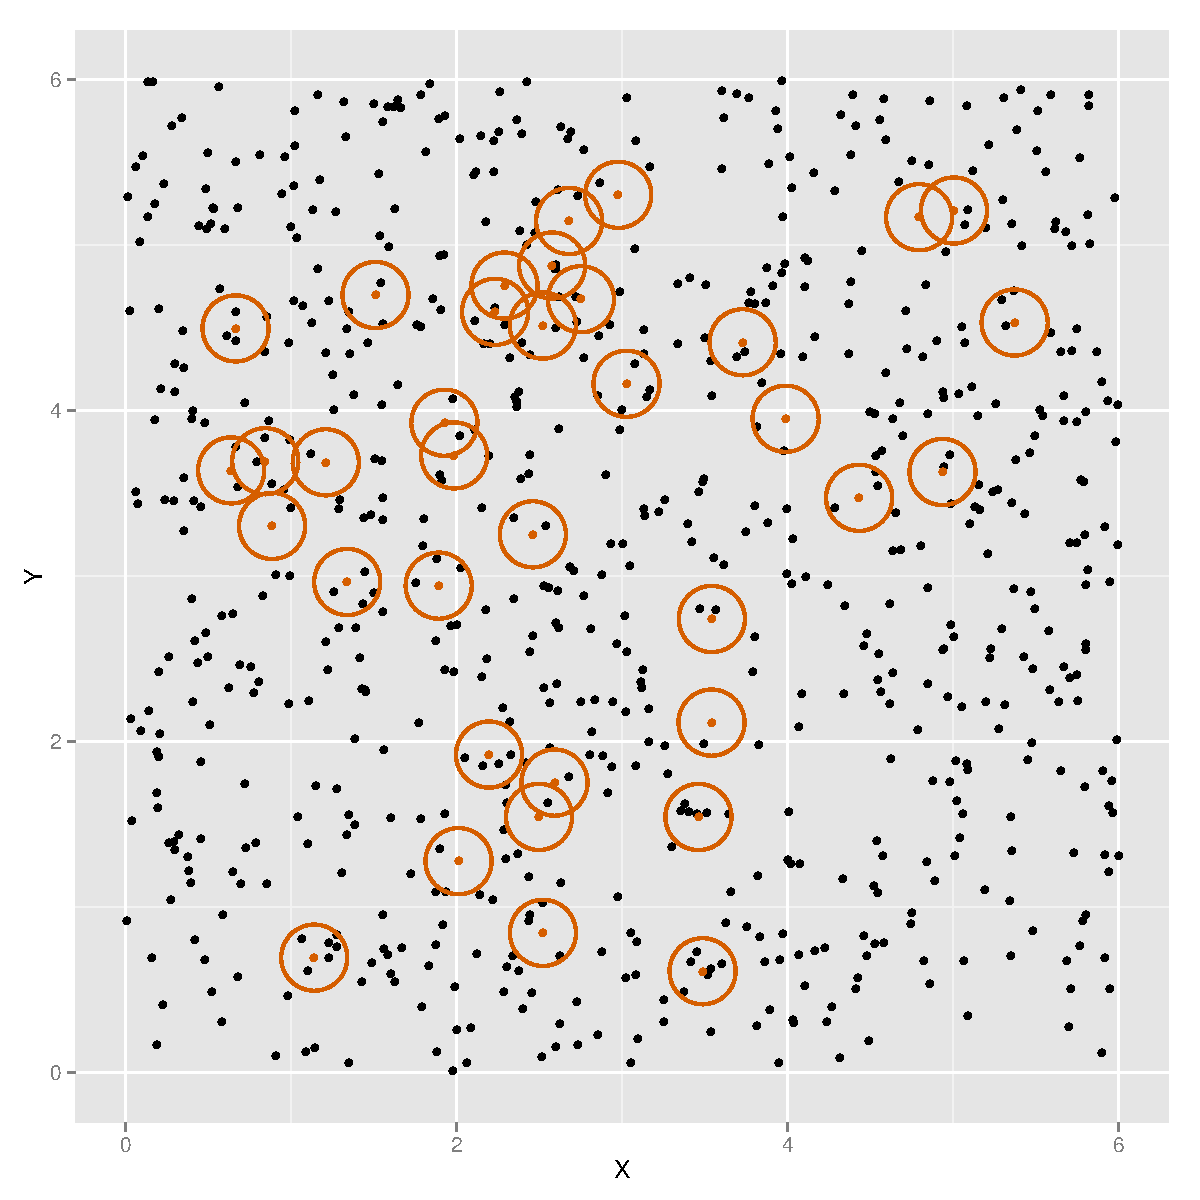
\includegraphics[width=\textwidth]{../images/layout_random.pdf}
		\caption{Totally Random Layout}
		\label{fig:random}
	\end{subfigure}
	
	\begin{subfigure}[b]{0.45\textwidth}
		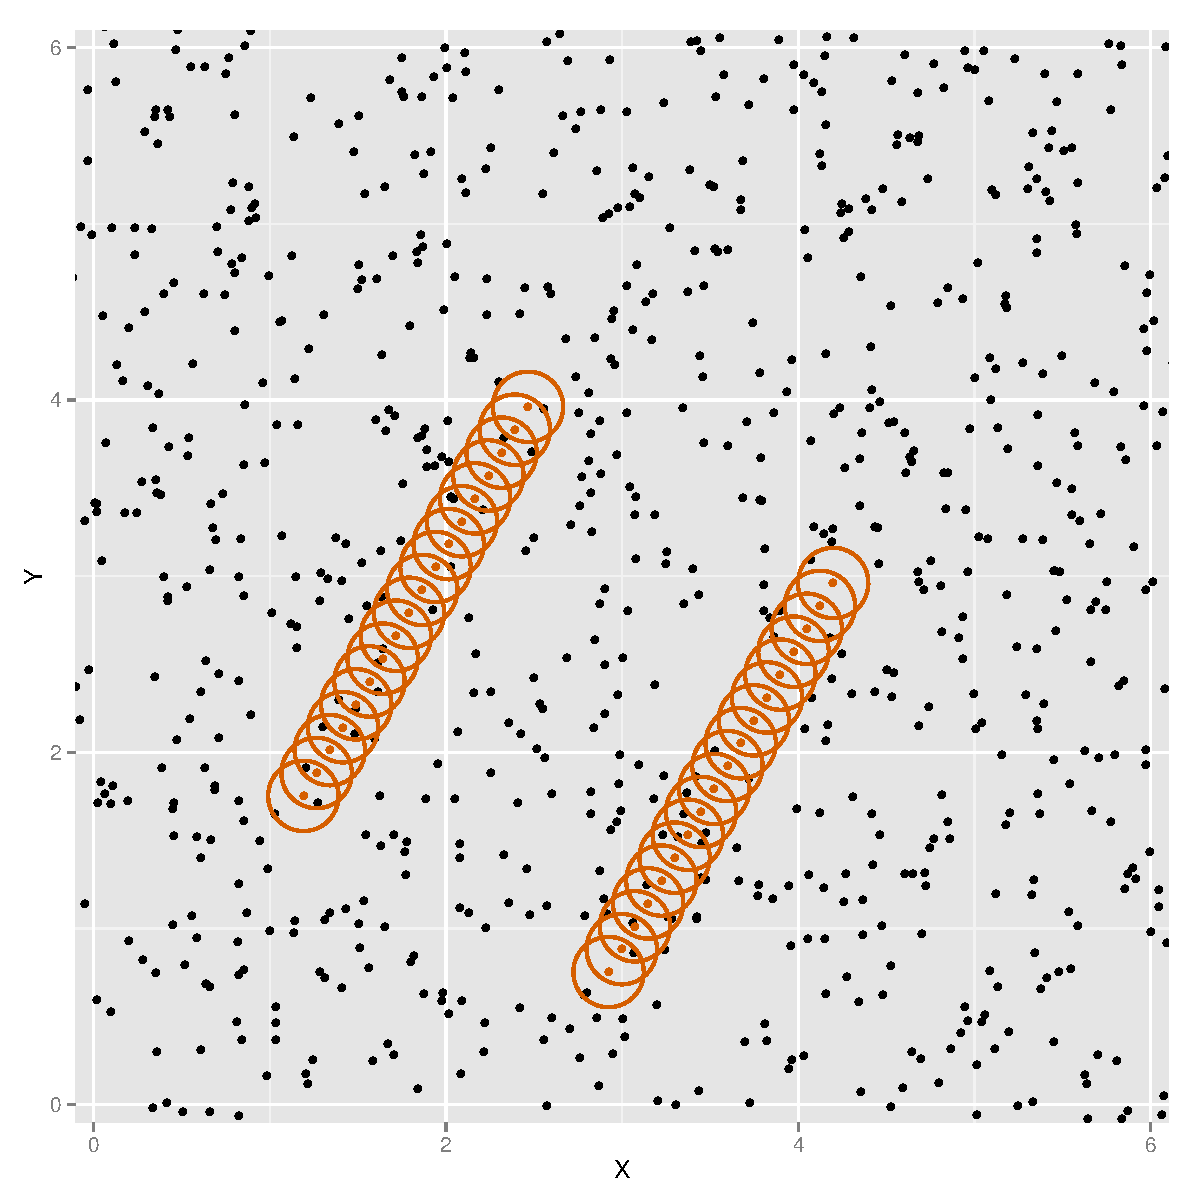
\includegraphics[width=\textwidth]{../images/layout_rand-sys-4.pdf}
		\caption{A Transect Layout}
		\label{fig:transect1}
	\end{subfigure}
	\begin{subfigure}[b]{0.45\textwidth}
		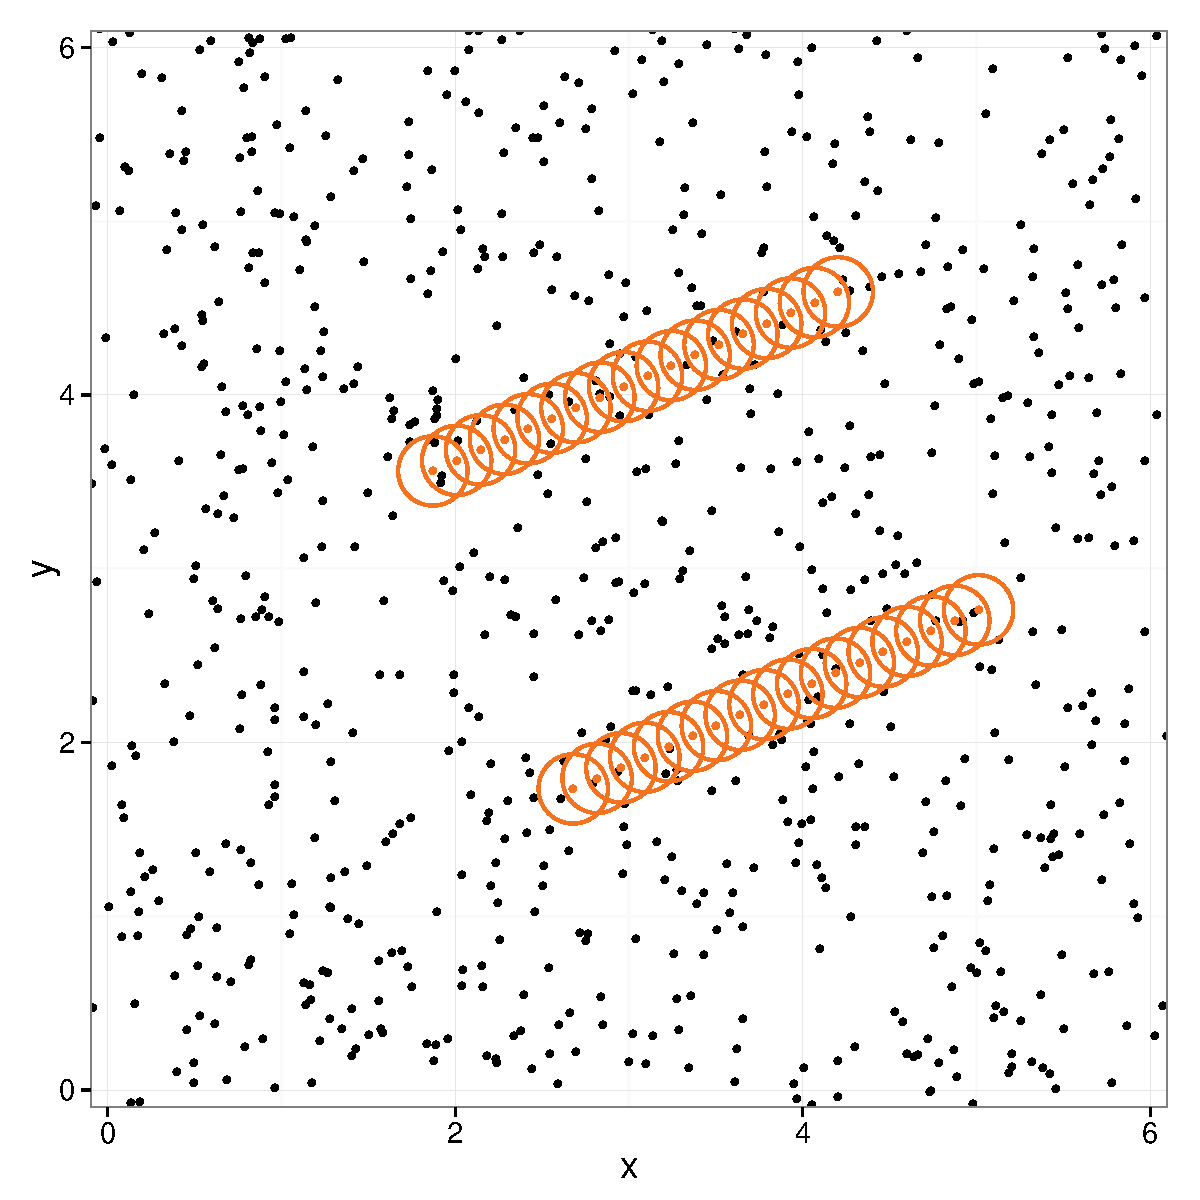
\includegraphics[width=\textwidth]{../images/layout_rand-sys-6.pdf}
		\caption{Another Transect Layout}
		\label{fig:transect2}
	\end{subfigure}
	\caption{VCP Layout options. On graph, 1 unit = 1 km. Circles represent 200 m mark.}
	\label{fig:layouts}
\end{figure}
Figures~\ref{fig:structured} and \ref{fig:random} illustrate the first two arrangements. Density in these images is based on the 20 birds per km$^2$ of the Palie region on Rota. 

As seen in Figure~\ref{fig:82dist}, there is very little detection happening beyond 500 m. There are a total of 15 observations beyond 500 m, which is 0.9\% of the data. 

The surveyed area of the Palie region totaled 9.41 km$^2$ during the original survey. Treating 500 m as our truncation distance $w$, the study area in the simulation has been raised from 9.41 km$^2$ to 36 km$^2$ to allow for stations where the observation area did not overlap. An area of 49 km$^2$ is generated with the given density, then truncated to 36 km$^2$ to prevent any edge effect from the random generation of points. The stations are placed a minimum of 500 km (0.5 on the graph) away from the edges to prevent border truncation. 

The Palie region contained two transects of 16 and 17 stations each, 33 stations total \parencite{micronesian}. For the transect layout, an angle was chosen between $0$ and $\pi$. A transect of 18 stations 150 m apart was constructed, and a second transect of 18 stations constructed running parallel. The transects were then randomly placed with in the graph, no closer to the edge than 500 km (0.5 on graph.) This transect layout is illustrated in Figures~\ref{fig:transect1} and \ref{fig:transect2}. The total of 36 VCPs was carried over to the Structured and Random layouts, for an equivalent number of points.

\subsection{Detection Probability Options}
The first simulation compares the three layouts described in section~\ref{sec:layout} with two different options for $g(r)$, a half-normal detection probability function, and a detection probability estimated from the empirical observation distances.
\subsubsection{Half Normal}
For a maximum possible observation distance of 0.500 (500 m), the parameter for the half-normal detection function is $\theta = 8.77$, with a scale parameter $\delta = 0.179$.

The half-normal parameter $\theta$ is related to the standard deviation of a standard normal distribution by the relationship:

$\theta = \dfrac{\sqrt{\pi /2}}{\sigma}$

If we estimate $\sigma$ by $w/3.5$ (with $w$ being the maximum distance at which we might observe an object, and 3.5 being the standard deviation point where $P(X > 3.5) < 0.001$) then $\theta$ is:

$\sigma = \dfrac{w}{3.5} = 0.1429$

$\theta = \dfrac{\sqrt{\pi /2}}{0.1429}=8.7732$

For a half-normal with parameter $\theta=8.7732$, $f(0)=5.5852$ so to scale the value to 1:
\begin{center}
$\delta_{HN} = \dfrac{1}{5.5852} = 0.1790$
\end{center}


Half-normal density functions were executed in R with the \texttt{fdrtool} package.
\begin{figure}
	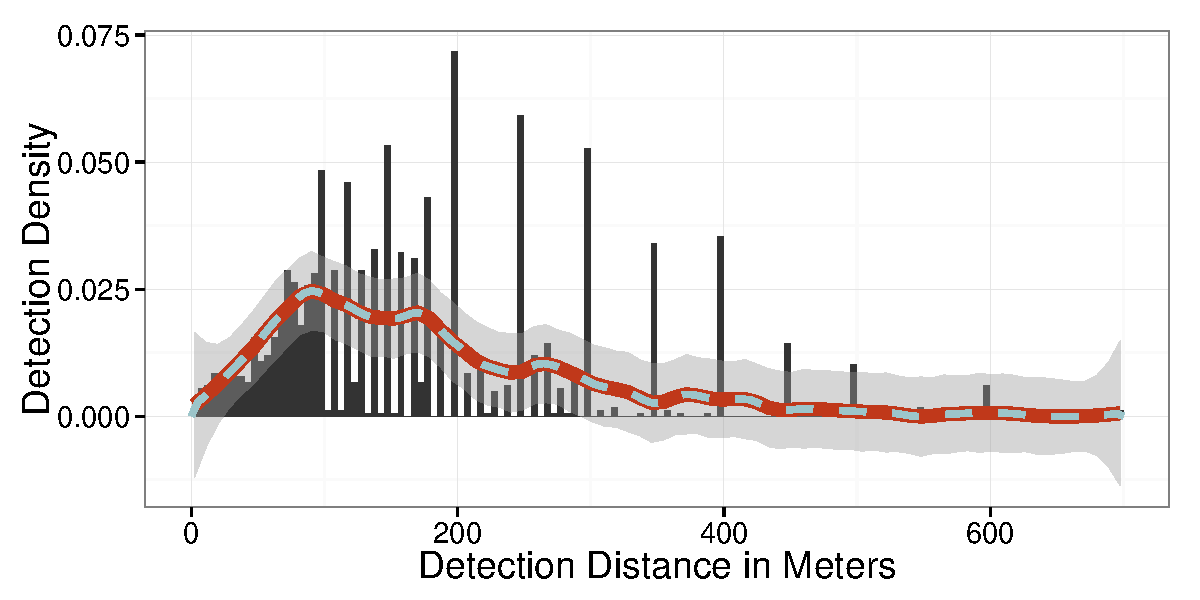
\includegraphics[width=\textwidth]{../images/loess.pdf}
	\caption{Empirical Observation Distances from Original data in meters, with LOESS regression lines. Bin width=5 m\label{fig:by5}}
\end{figure}
\subsubsection{Empirical Observations}
Figure \ref{fig:by5} illustrates that above 100 m, observations were commonly heaped into 10 or 25 m distances, with the latter being more heavily used. Above 200 m, 50 m heaps were common. 

Using the \texttt{hist()} function in R, the 1982 observation distances were broken into counts by 5 m groups. Using the bin midpoints, the density estimate was multiplied by 5 to get the density value for that bin. A LOESS regression was run with the midpoint as $x$ and $y=density*5$, using the \texttt{loess()} package in R with a span of 0.2. This is the solid line in Figure~\ref{fig:by5}. 

This gives us an object that can be used with \texttt{predict()} to get density estimates for specific distances. The values generated by feeding our midpoints into our prediction function are represented by the dashed line in Figure~\ref{fig:by5}. 

Following the scaling of the highest point to 1, as was done with the half normal curve, where the highest point was $g(0)$, we also find $\delta$ for this empirical detection probability. A sequence of $x$ values was generated covering the range from 0--500 m. This was plugged into the \texttt{predict()} function using our LOESS object. The highest density value was then scaled to be 1:

$\delta_{EMP}=\dfrac{1}{max(predicted)}=40.5780$ 

\subsubsection{Movement}
In the Figure~\ref{fig:82dist}, the histogram of empirical observation distances, there appears to be evidence of movement away from the observer. To see if the movement would have an effect on the independence of our VCPs, depending on placement, a second simulation was run.

Three movement classes were defined:
\begin{enumerate}
\item No Movement: Objects stayed at original point.
\item Temporary Movement: Objects within 100 m had a random chance to move directly away from observer. Movement was larger if they started closer to observer. They were reset to original location before moving to next VCP
\item Permanent Movement: As with temporary movement, only not reset before moving on to next VCP. (Movement could compound if object was within the maximum observation radius for more than one VCP.)
\end{enumerate}

For this simulation, the movement was simulated to happen within the first 100 m from the observer (0.1 on graph), as visually indicated by Figure~\ref{fig:82dist}. The simulation was not intended to exactly model the movement observed by \textcite{micronesian}, but to get a general sense of what might happen to $\hat{D}$ in each of the two settings.

\section{Results}
Two simulations were run, one looking at the three layout options crossed with the two detection probability function options and the other examining the effect of the three layout options against the three movement options, holding the detection probability option standard.
\subsection{Half-normal vs. Empirical $g(r)$}
\begin{figure}

	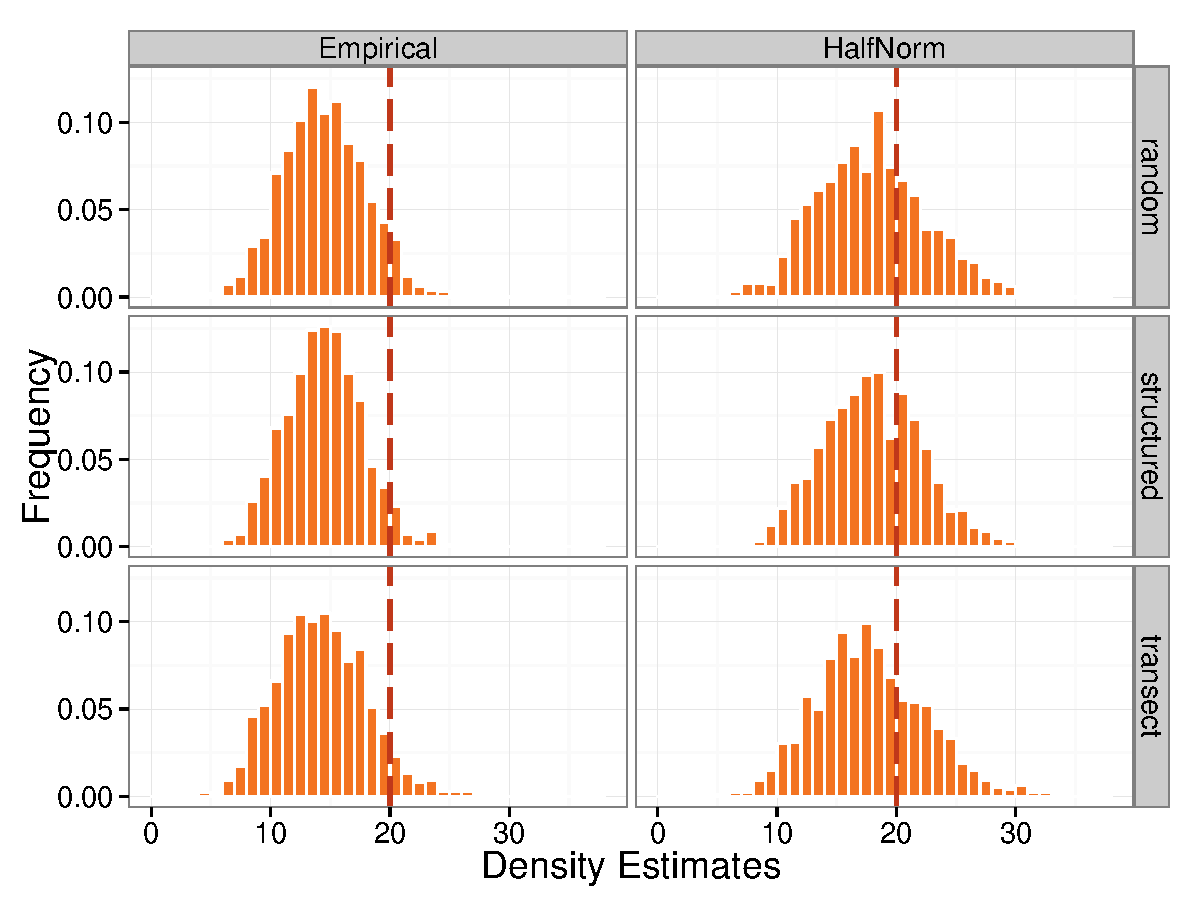
\includegraphics[width=\textwidth]{../images/Emp_Vs_Hnorm_1-2.pdf}
	\caption{1000 Simulations, Empirical vs Half-normal Detection function, for three different layouts. Dashed line equals true value of 20 objects per km$^2$\label{fig:sim1}}
		
\end{figure}
Figure \ref{fig:sim1} shows the results of 1000 simulations, each analyzed with Empirical and Half-normal detection function, $g(x)$, and using each of the three layouts, Structured, Random, and Transect. All $\hat{D}$  were done using the kernel method with a normal kernel \parencite{quang1993}.

For each simulation, a single layout of ``objects'' is generated, and that map is analyzed by each of the 6 combinations of VCP layout and $g(x)$. 

As we would expect, the density estimates using $g(x)$ based on the Empirical distance observations is biased low. We also see bias in the estimates using the half-normal function for $g(x)$, but it is much less severe than in the Empirical data. \textcite{quang1993} does provide a bias-correction method, but it was not used for this simulation.

Addressing our primary question of interest, does the overlap of the VCP affect the population density estimate due to violation of independence, the answer would appear to be no. Looking at the simulations with the Half-normal detection function, the histograms are fairly similar across the three layouts. 

Table~\ref{table:sim1} supports what we observe in the histogram: the centers vary between our two $g(r)$ options, but are approximately the same within the each option, regardless of which VCP layout we have chosen. Table~\ref{table:sim1capture} shows the percentage of simulations that captured the true object density of 20 per km$^2$ within a 95\% confidence interval. \cite{quang1993}

There may be evidence of a drop in accuracy with the Transect layout, but it is difficult to determine if this is a valid observation, or an artifact of this particular simulation. The drop, if it exists, is much less severe with the half-normal detection function. With the empirical detection function, the structured layout percentage swings much higher than the result from our random layout, unlike for half-normal where they are just over 1\% apart. Repeated simulations, could help narrow down if this is a true effect, or simply random noise.
\begin{table}[h]

	\begin{tabular}{ r r |r r| r r r}
		$g(x)$      & Layout     & Mean  & Std Dev & 25th  & Median & 75th  \\ \hline\hline
		Empirical   & Random     & 14.47 & 3.37    & 12.08 & 14.38  & 16.73 \\
		Empirical   & Structured & 14.49 & 3.15    & 12.27 & 14.47  & 16.59 \\
		Empirical   & Transect   & 14.26 & 3.66    & 11.65 & 14.14  & 16.80 \\ \hline
		Half-normal & Random     & 17.90 & 4.57    & 14.67 & 17.86  & 20.88 \\
		Half-normal & Structured & 18.03 & 4.16    & 15.05 & 17.91  & 20.82 \\
		Half-normal & Transect   & 17.80 & 4.64    & 14.52 & 17.44  & 20.78
	\end{tabular}
	\caption{Centers and Spread for Empirical vs. Half-normal detection functions. 1000 simulations. True density 20/km$^2$}
	\label{table:sim1}
\end{table}
\begin{table}[h]

	\begin{tabular}{ r| r r| r r|}
		           & \multicolumn{2}{|c|}{Empirical} & \multicolumn{2}{|c|}{Half Normal} \\ \hline\hline
		Layout     & Mean $\hat{D}$ & \% Capture     & Mean $\hat{D}$ & \% Capture       \\ \hline\hline
		Random     & 14.47          & 73.6\%         & 17.90          & 94.0\%           \\
		Structured & 14.49          & 77.5\%         & 18.03          & 95.3\%           \\
		Transect   & 14.27          & 69.6\%         & 17.80          & 91.2\%           \\ \hline
	\end{tabular}
	\caption{True Density Capture, Emperical vs. Half-normal detection function for three layouts. 1000 simulations.}
	\label{table:sim1capture}
\end{table}

\subsection{Movement or No Movement}
\begin{figure}

	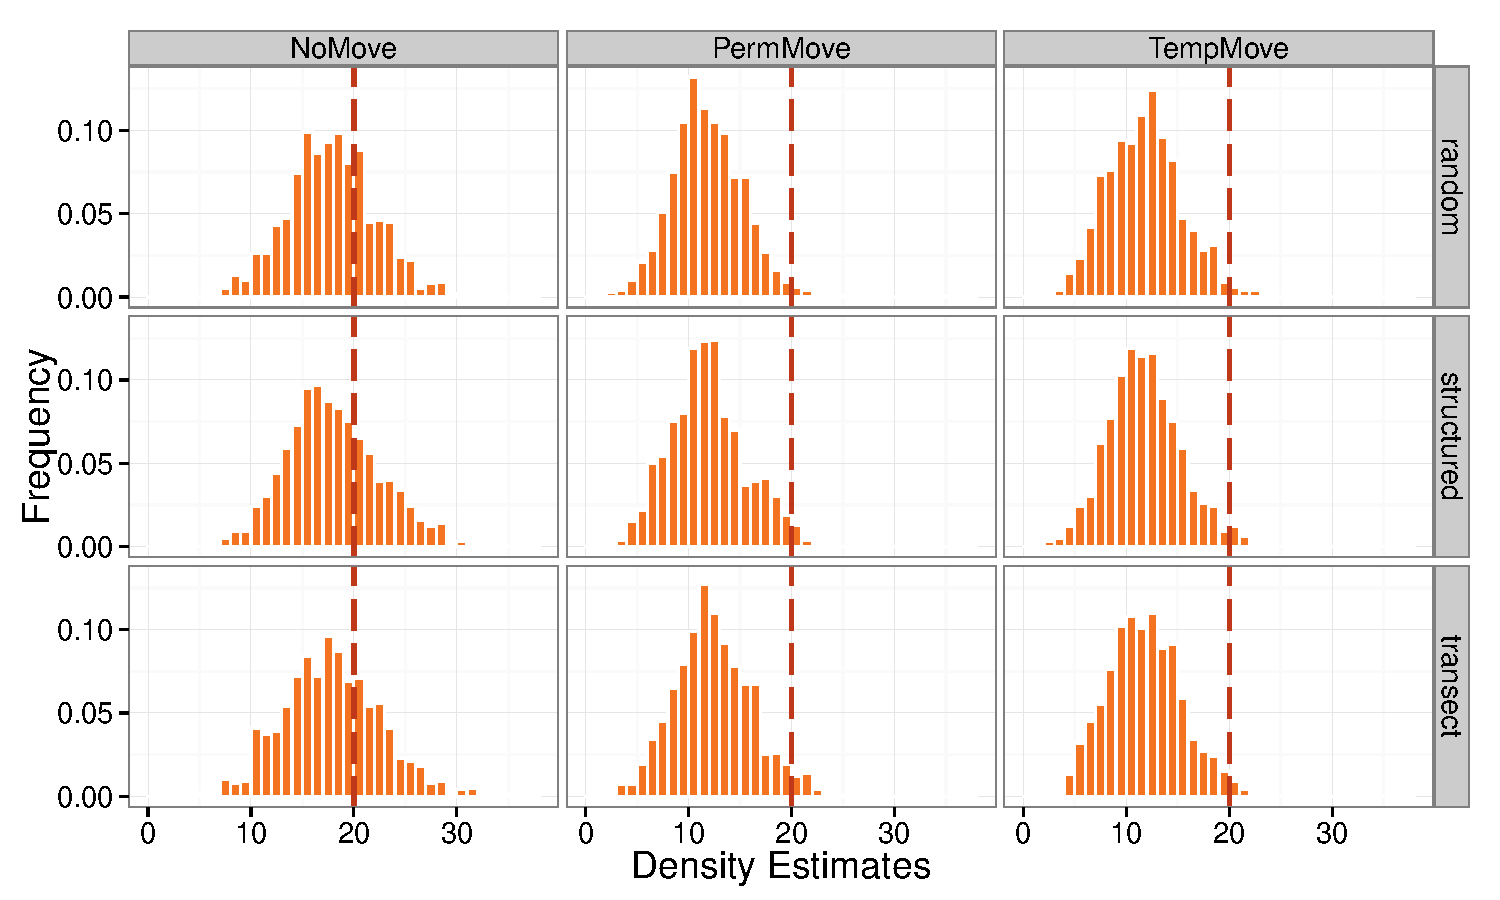
\includegraphics[width=\textwidth]{../images/MovementSim2.pdf}
	\caption{1000 Simulations, Movement, Temporary Movement and Permanent Movement for three different layouts. \label{fig:sim2}}
		
\end{figure}
\begin{table}[h]

	\begin{tabular}{ r r| r r| r r r}
		Movement  & Layout     & Mean  & Std Dev & 25th  & Median & 75th  \\ \hline\hline
		None      & Random     & 17.86 & 4.28    & 15.03 & 17.64  & 20.65 \\
		None      & Structured & 18.01 & 4.51    & 14.95 & 17.62  & 20.94 \\
		None      & Transect   & 17.90 & 4.78    & 14.74 & 17.67  & 20.95 \\ \hline
		Permanent & Random     & 11.86 & 3.42    & 9.58  & 11.61  & 14.09 \\
		Permanent & Structured & 11.90 & 3.65    & 9.37  & 11.67  & 14.08 \\
		Permanent & Transect   & 12.42 & 3.72    & 9.93  & 12.17  & 14.79 \\ \hline
		Temporary & Random     & 11.76 & 3.57    & 9.22  & 11.75  & 14.02 \\
		Temporary & Structured & 11.74 & 3.48    & 9.37  & 11.56  & 13.85 \\
		Temporary & Transect   & 11.75 & 3.57    & 9.24  & 11.72  & 14.20
	\end{tabular}
	\caption{Centers and Spread for Movement and Layout combinations. 1000 simulations. True density 20/km$^2$}
	\label{table:sim2}
\end{table}
\begin{table}

	\begin{tabular}{ r| r r| r r| r r|}
	
		& \multicolumn{2}{|c|}{No Movement}	& \multicolumn{2}{|c|}{Compounded Mvmt}	& \multicolumn{2}{|c|}{Temporary Mvmt}\\ 
 \hline \hline
 
 Layout		& Mean $\hat{D}$	& \% Capture & Mean $\hat{D}$ & \% Capture & Mean $\hat{D}$ & \% Capture	\\ \hline \hline
 Random		& 17.86 			& 94.2\% 		& 11.86	& 59.6\%	& 11.76	& 59.3\% \\
 Structured	& 18.01 			& 94.3\% 		& 11.90 & 59.9\% 	& 11.74 & 59.5\% \\
 Transect	& 17.90 			& 90.8\% 		& 12.42 & 65.0\% 	& 11.75 & 58.0\% \\ \hline

	\end{tabular}
	\caption{Mean and Capture Rate, Half-normal detection function, three layouts, three movement types. 1000 simulations.}
	\label{table:sim2capture}
\end{table}

Figure~\ref{fig:sim2} and Tables~\ref{table:sim2} and~\ref{table:sim2capture} illustrate the results of our movement type simulation. For this run, only the half-normal detection function was used. 

For testing combinations of movement and VCP layout, only the half-normal detection function was utilized. Figure~\ref{fig:sim} compares the histograms of the nine combinations. On the whole, the estimates are biased low, as was observed in the previous simulation, without movement. Within a column, the results are fairly similar in shape and spread. The most obvious differences lie between columns, indicating that the type of movement causes more bias in our estimate than the potential overlap of our observation areas. 

Table~\ref{table:sim2} reinforces this conclusion, as the measures of center and spread are reasonably consistent within Movement type, regardless of the VCP Layout. Differences are observed between movement types, with No Movement having the estimates with the smallest amount of downward bias, and Compounded and Temporary movement biasing the population density estimate about the same amount.

Unexpectedly, the type of movement, temporary or permanent, does not seem to play a large part in changing the bias. Table~\ref{table:sim2capture} shows that the 95\% confidence intervals \parencite{quang1993} capture the true mean about 59\% of the time, no matter which movement type, Temporary or Compounded.

The similarity for the Structured and Random layouts can be explained by a general lack of compounded movement. For the Structured layout, the animals would only move once, additional movement would not be triggered by an overlapping VCP, so the Compounded Movement setting would have the same end result as the Temporary Movement setting. For the Random VCP layout we would expect there to be a larger effect from the Compounded movement, because we will have VCPs whose observation distances overlap. 

Looking at Figure~\ref{fig:random}, which is just one possible random layout, there are 8 pairs of VCP where the circles representing the 200 m mark overlap, and 3 where they overlap to any significant degree. With most of the movement happening within that first 100 m, we would expect the estimate to be fairly similar to the Structured layout setting, if this random layout is typical of those generated. 

The combination of compounded movement and the transect layout seems to have an effect on the density estimate. The other estimates for either movement type, are all in the same ballpark, around 11.8 with an approximate 59\% rate for capturing the true population value. For the Transect Layout and Compounded movement, this rises 0.50 to a mean population density estimate of 12.42, and a capture percent of 65\%. It is unclear if there is something about this combination that is reducing bias (possible, but feels unlikely), or if it is instead biasing the estimate upwards, which appears like bias reduction because the estimate is already low.

%\texttt{TODO: Try to xplain the .50 jump in the estimate for transect/compounded. No theory or story atm.}

%NOTE: no small distances, so overestimating area surveyed compared to \# ob
%NOTE: we will be low if top small, bottom large.

\section{The Problem with Circles}
To test the effectiveness of the movement algorithm, the detection distances from the data where the objects moved was compared to the detection distances from the same data, assuming the objects stayed still. The movement data, (left panel, Figure~\ref{fig:moveTest}) is squashed more towards 0.1 Km than the still data (right panel). But there is a problem. The still data does not show the nice shoulder at 0 that the literature instructs us to expect.

\begin{figure}[h]
	\center
	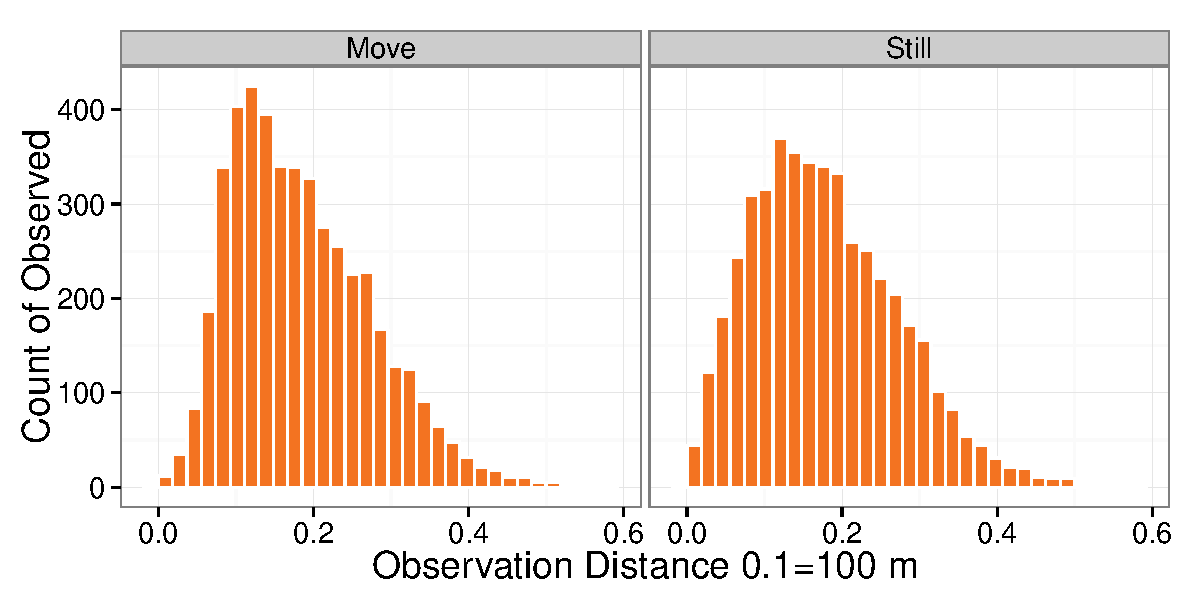
\includegraphics[width=\textwidth]{../images/movementTest.pdf}
	\caption{Simulated bird distances from center point of 36 randomly placed VCPs.\label{fig:moveTest}}
\end{figure}

The problem is because circles are different than rectangles. With a line transect, as we move away from the line an equal distance in either direction, the distance surveyed increases linearly. With a point transect, as we move away from the point, the distance surveyed increases exponentially. Figure~\ref{fig:perfectArea} shows the relationship for a rectangle and circle with the same area. 

Figure~\ref{fig:perfectCount} shows the difference in the expected number of observed objects at distance $r$ given a line transect vs. a VCP. For the VCP, Area was calculated as $2\pi r$. For the line transect, Area was calculated as $(2r)L$, with $L=0.785$ chosen so that the area of the circle and rectangle were equal when $r=0.5$.

$E[observed] = Area*Density*P(\mbox{object observed}|\mbox{distance }r)$

The take-away point is that for a VCP survey, even if everything is perfect, the empirical detection distances will not show the nice shouldered layout of the ideal detection probability curve. \textcite{ramsey1981} speak about this, when comparing the ``CUM-D'' curve, or the plot of the cumulative number of observations at distance $r$ for both line and point transects. However, almost all the illustrations on how the collected data should look, shows data that echoes the detection probability curve: the half-bell-shape with a nice shoulder. Since this shape is impossible for VCP, explicit examples should be shown in the literature so researchers do not assume their is something wrong with their data.

Many researchers have worked on distance sampling, and this effect is taken into account in the calculation of population density estimates. When analyzing point transect data we take the derivative of $g(r)$, an adjustment which is not necessary in line transect surveys. It can be shown that this solution adjusts for the difference in how area is calculated, to result in correct density estimates. 

%Thought - is this why we use h(0) for the point transects? need to verify, h(r) = f'(r)??  budkland 1987 paper has h(r) = f(r)/r, need to check teh book.  - yes.

\begin{figure}
	\centering
	\begin{subfigure}[b]{0.45\textwidth}
		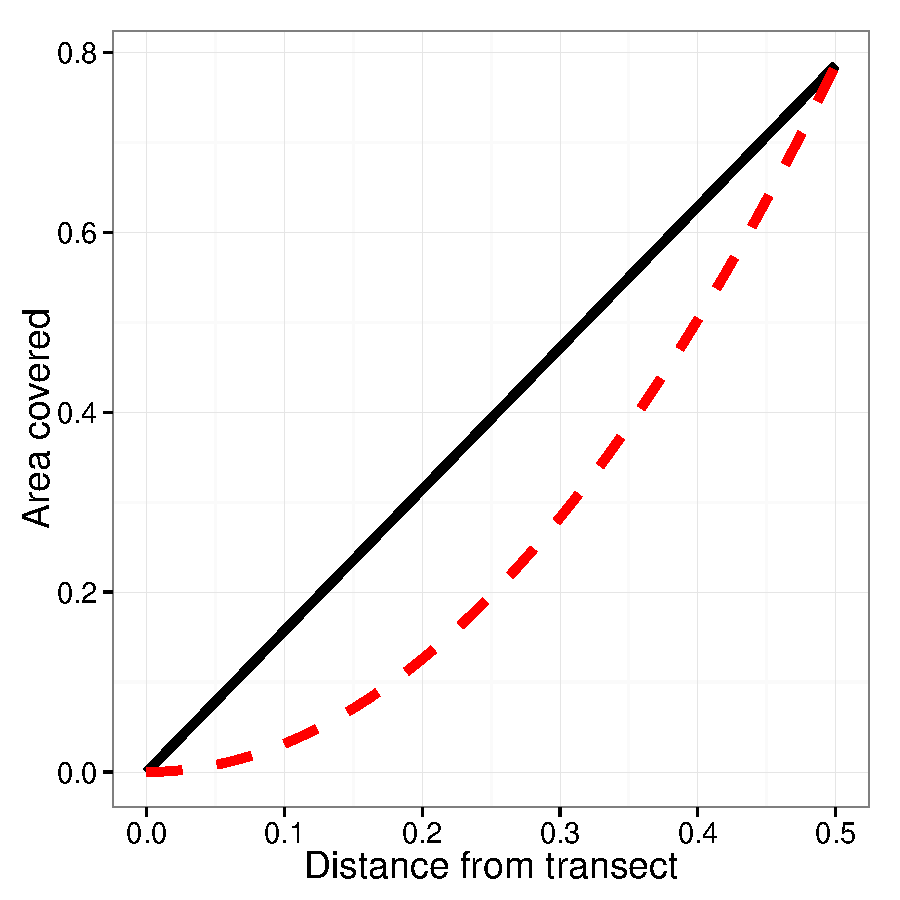
\includegraphics[width=\textwidth]{../images/rect-circ-area.pdf}
		\caption{Area of rectangle vs circle at same distance from point/line}
		\label{fig:perfectArea}
	\end{subfigure}
	\begin{subfigure}[b]{0.45\textwidth}
		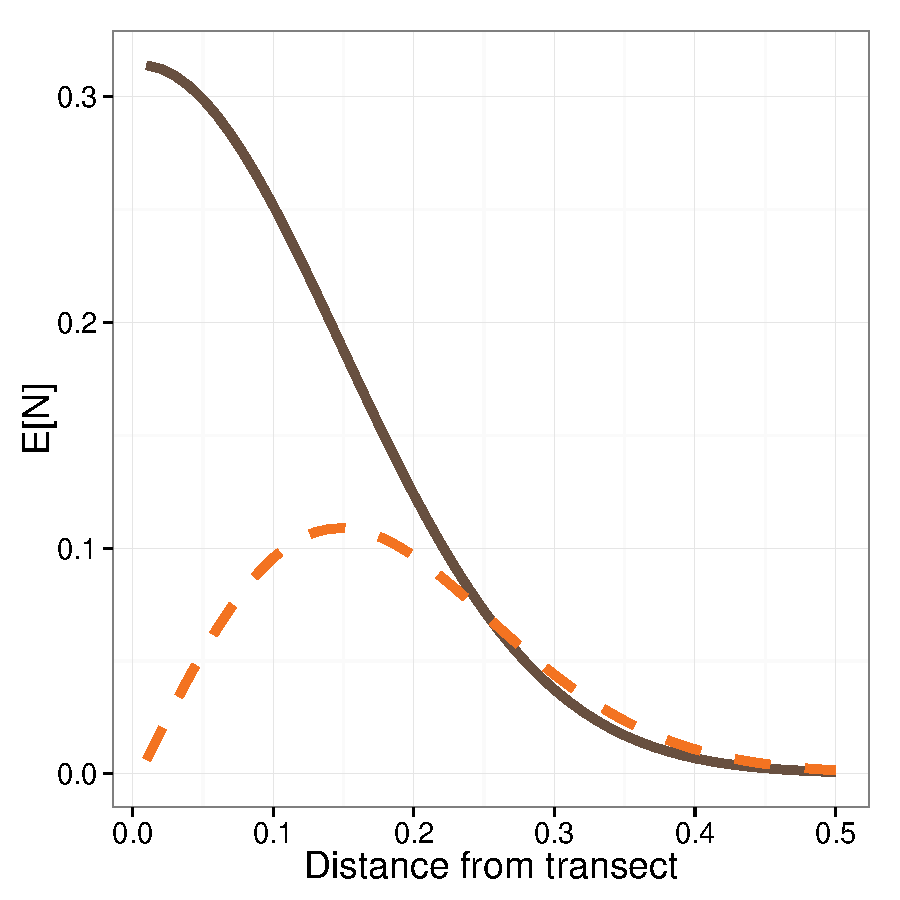
\includegraphics[width=\textwidth]{../images/rect-circ-detection.pdf}
		\caption{Estimated detection numbers for rectangle (solid) vs circle (dashed)}
		\label{fig:perfectCount}
	\end{subfigure}
	\caption{Rectangles (Line Transect, solid) vs. Circles (Point Transect, dashed)}
	\label{fig:linevs}
\end{figure}


\section{Conclusions}
If all else is held equal, VCP layout does not seem to play a large role in population density estimates using the kernel method as described by \textcite{quang1993}. Violations of the expected detection probability curve, or by movement of the objects away from the observer play more of a role in biasing the resulting estimate. 

All of the population density estimates were biased low using Quang's formula for $\hat{D}$. This bias was observed even when the detection function was a half-normal curve and analyzed with a normal kernel, and the VCPs were placed so that the observation area did not overlap. The bias was not severe in this case, it estimated a population density around 18 objects per km$^2$, when the true estimate was 20/km$^2$, but it is noticeable. Dr. Quang's paper does offer a bias-corrected estimate, which was not used in this simulation. 

There is a possible effect of the combination of compounded movement and the transect layout. It is unclear from these results what the particular cause of the increased estimate and accuracy is. Future work might involve modification of the simulation functions to return more information, such as the count of observed animals and the observation distances to assist with understanding why this combination is producing an estimate that appears out of line with it's neighbors.


%\section{Bibliography}

\printbibliography
%\bibliographystyle{plain}
%\bibliography{VCPbibliography}
\end{document}